\documentclass{standalone}

\usepackage{tikz}
    \usetikzlibrary{arrows.meta}
    \usetikzlibrary{calc}
    \usetikzlibrary{decorations.pathmorphing}

\tikzset{
    greensq/.style={
        green,
        fill=green!20, 
        line width=0.4mm,},
    redsq/.style={
        red,
        fill=red!5, 
        line width=0.4mm,},
    }
    
\begin{document}
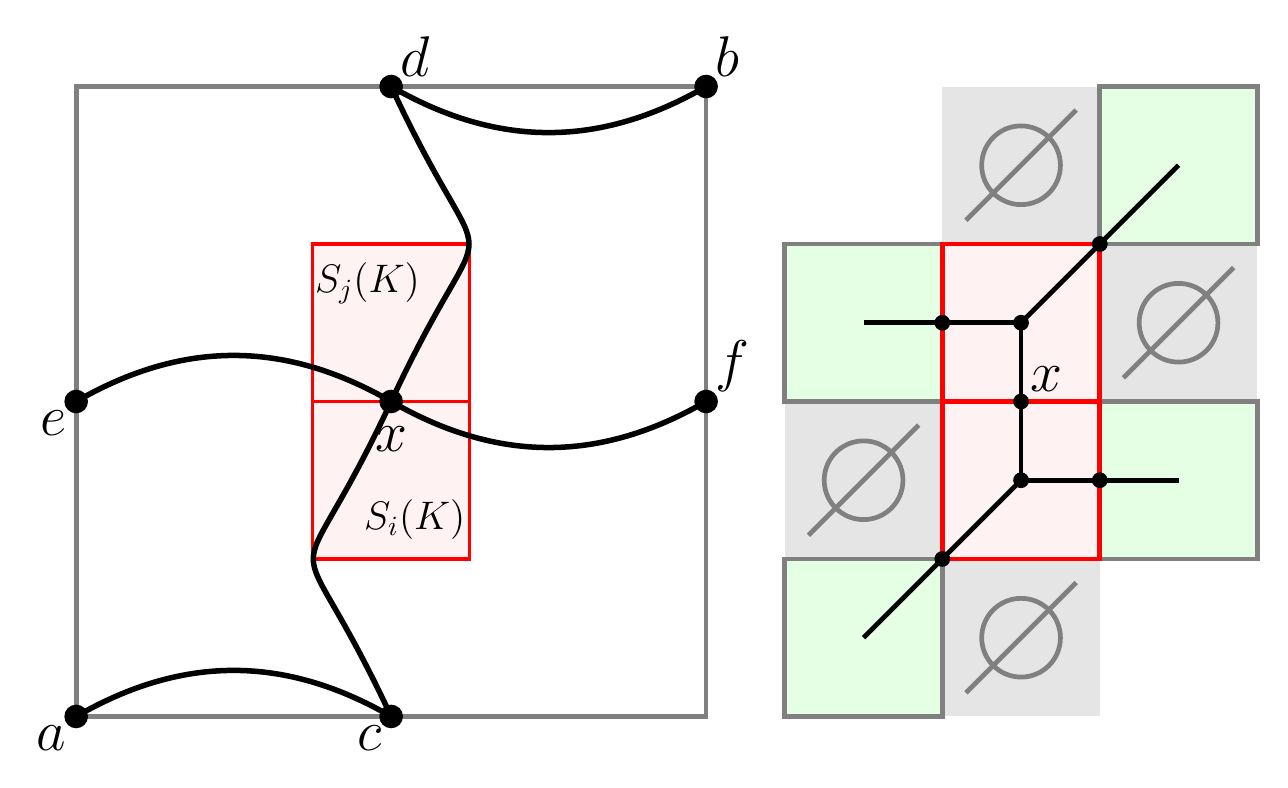
\begin{tikzpicture}
    % \draw[help lines] (0,0) grid (15,3);
    \draw[black!50, line width=0.6mm] 
        (0,0) rectangle(8,8);
    \foreach \x in
        {(3,2), (3,4)} 
        {\draw[redsq] \x rectangle+(2,2);}
    \foreach \x in
        {(9,2), (11,0), (11,6), (13,4)} 
        {\fill[black!10] \x rectangle+(2,2);
         \draw[black!50, line width=0.6mm,] 
            \x++(0.3,0.3) -- +(1.4,1.4)
            \x++(1,1)circle(0.5);}
    \foreach \x in
        {(9,0), (13,2), (9,4), (13,6)} 
        {\draw[black!50, line width=0.6mm, fill=green!10] 
            \x rectangle+(2,2);}
    \foreach \x in
        {(11,2), (11,4)} 
        {\draw[redsq, line width=0.6mm] 
            \x rectangle+(2,2);}
    \path[line width=0.7mm]
        (4,4) edge[bend right] +(4,0)
              edge[bend right] +(-4,0)
              edge[bend right=25, looseness=2] +(0,4)
              edge[bend right=25, looseness=2] +(0,-4)
        (0,0) edge[bend left] +(4,0)
        (4,8) edge[bend right] +(4,0);
    % \path[line width=1mm, cyan!40]
    %     (12,3) edge[bend right] +(1,0)
    %            edge[bend right] +(-1,0)
    %            edge[bend right=25, looseness=2] +(0,1)
    %            edge[bend right=25, looseness=2] +(0,-1)
    %     (11,2) edge[bend left] +(1,0)
    %     (12,4) edge[bend right] +(1,0)
    %     (12,5) edge[bend right] +(1,0)
    %            edge[bend right] +(-1,0)
    %            edge[bend right=25, looseness=2] +(0,1)
    %            edge[bend right=25, looseness=2] +(0,-1)
    %     (11,4) edge[bend left] +(1,0)
    %     (12,6) edge[bend right] +(1,0);
    \path[line width=0.6mm]
        % (10,2) edge[bend right] +(1,0)
        % (14,3) edge[bend right] +(-1,0)
        % (12,3) edge[bend right] +(1,0)
        %        edge[bend right=25, looseness=2] +(0,1)
        %        edge[bend right=25, looseness=2] +(0,-1)
        % (11,2) edge[bend left] +(1,0)
        % (10,5) edge[bend right] +(1,0)
        % (12,5) edge[bend right] +(-1,0)
        %        edge[bend right=25, looseness=2] +(0,1)
        %        edge[bend right=25, looseness=2] +(0,-1)
        % (13,6) edge[bend left] +(1,0)
        % (12,6) edge[bend right] +(1,0)
        % (14,6) edge[bend left=25, looseness=2] +(0,1)
        % (10,2) edge[bend left=25, looseness=2] +(0,-1)
        (12,3) edge +(0,2)
               edge +(-2,-2)
               edge +(2,0)
        (12,5) edge +(-2,0)
               edge +(2,2);
    \foreach \x in
        {(0,0), (4,0), (8,8), (4,8), (8,4), (0,4), (4,4)}
        {\fill[black] (\x circle (1.5mm);}
    \foreach \x in
        {(11,2), (12,3), (12,4), (13,3), (11,5), (13,6), (12,5)}
        {\fill[black] (\x circle (1mm);}
    \node at (4.3,2.5) {\Large$S_i(K)$};
    \node at (3.7,5.5) {\Large$S_j(K)$};
    \node[below left] at (0,0) {\huge$a$};
    \node[above right] at (8,8) {\huge$b$};
    \node[below left] at (4,0) {\huge$c$};
    \node[above right] at (4,8) {\huge$d$};
    \node[below left] at (0,4) {\huge$e$};
    \node[above right] at (8,4) {\huge$f$};
    \node[below=2mm] at (4,4) {\huge$x$};
    \node[above right] at (12,4) {\huge$x$};
    % \node[below left] at (11,3) {\large$S_i(e)$};
    % \node[shift={(-0.2,-0.4)}] at (12,2) {\large$S_i(c)$};
    % \node[above right] at (15,5) {\large$S_j(f)$};
    % \node[shift={(0.2,0.4)}] at (14,6) {\large$S_j(d)$};
    % \draw [->,>={Latex[length=3mm]}, line width=0.5mm]
    %     node at (15,1) {\Large$S_i(x)$} 
    %     edge[bend right=15] (12.2,2.9);
    % \draw [->,>={Latex[length=3mm]}, line width=0.5mm]
    %     node at (11,7) {\Large$S_j(x)$} 
    %     edge[bend right=15] (13.8,5.1);
\end{tikzpicture}
\end{document}